% !TeX spellcheck = pt_BR
% !TeX encoding = UTF-8
% !TeX program = pdflatex
%---
% Template para LaTeX de Artigo para submissão na ANPET
% Customização por lgscarvalho@usp.br
% Texto adaptado de artigo disponível em: http://anpet.org.br/ssat/interface/content/autor/arquivos/formato_trabalhos.doc
% Código adaptado do proposto por Berg Dantas, disponível em: http://docente.ifrn.edu.br/julianaschivani/disciplinas/midias-educacionais/latex-modelo-para-artigo-cientifico-de-acordo-com-a-abnt/view
%---
\documentclass[article,12pt,a4paper,oneside,hidelinks]{memoir}		
% Pacotes usados
\usepackage[T1]{fontenc}%Selecao de codigos de fonte.
\usepackage[utf8]{inputenc}%Codificacao do documento
%\usepackage{mathptmx}	% texto em Times
\usepackage[brazil]{babel}

\usepackage[largesc]{newtxtext} %
\usepackage[varqu,varl]{zi4}% inconsolata
%\usepackage{cabin}% sans serif
\usepackage[scaled=.85]{helvet}		% sem serifa Helvetica
\usepackage[vvarbb]{newtxmath}

%\usepackage{indentfirst}%Indenta o primeiro parágrafo de cada seção.
%\usepackage{nomencl}%Lista de simbolos
\usepackage{color}%Controle das cores
\usepackage{graphicx}%Inclusão de gráficos
%\usepackage{microtype}%Para melhorias de justificação
%%\usepackage{lipsum}%Para geração de dummy text
\usepackage{hyperref}
%\usepackage[natbibapa]{apacite} % modificações nos comandos a seguir
%% definições para apacite
%	\renewcommand{\BCBT}{}  % retira a , entre 2 autores
%	\renewcommand{\BCBL}{}  % sem , entre os dois últimos autores
%	\renewcommand{\BBAA}{e}  % de & para "e" entre autores
%	\renewcommand{\BBAB}{e}  % de & para "e"
%	\renewcommand{\BAnd}{e}  % de & para "e"

\usepackage[square]{natbib}
%% o arquivo chicago-br.bst deve estar no mesmo diretório

\usepackage{nameref}
\usepackage{titlesec}%Customização de seções
\usepackage{caption} %Opções para chamadas de s e tabelas
\usepackage{enumitem} %Customização de listas
\usepackage{amssymb} %Símbolos matemáticos
\usepackage{amsfonts}
\usepackage{geometry} %Customização de dimensões da página
%\usepackage{soul} %Permite destacar texto e outras funções
%\usepackage{textgreek} %
%\usepackage{dsfont} %Fonte para grupos numéricos
\usepackage[table]{xcolor} %Facilita uso de cores
%\usepackage{graphbox} %Maior customização do posicionamento de figuras
%\usepackage{tikz} %Check mark
\usepackage{multicol}
\usepackage{multirow}

\usepackage{siunitx}
\usepackage{pifont}
\usepackage{xcolor}
\definecolor{ao}{rgb}{0.0, 0.5, 0.0}
\definecolor{bred}{rgb}{0.8, 0.0, 0.0}

\newcommand{\cmark}{\ding{51}}%
\newcommand{\xmark}{\ding{55}}%



\usepackage{relsize}
%Configuracoes do documento
\graphicspath{{./Figuras/}}%Images na pasta "Figuras"

%Configurações do texto das seções
\setsecheadstyle{\bfseries \normalsize \uppercase}
\setsubsecheadstyle{%
	\bfseries
	\normalsize}
\setsubsubsecheadstyle{\itshape \normalsize}
%Fim das configurações do texto das seções

% Configurações de parágrafo e espaçamento
\setlength{\parindent}{0pt} %paragrafo
\setlength{\parskip}{12pt}
\setlength{\baselineskip}{0pt}
\SingleSpacing
% Fim das configurações de parágrafo e espaçamento

% Configuração da legenda de figuras e tabelas
\captionsetup[figure]{labelfont={bf},labelsep=colon,skip=8pt,belowskip=-8pt,margin=1em,format=hang} 
\captionsetup[table]{labelfont={bf},labelsep=colon,skip=8pt,belowskip=-8pt,margin=1em,format=hang}

% Configuração da enumeração das seções.
\setsecnumdepth{subsubsection}
\titlelabel{\thetitle.  \ }
\titlespacing{\section}{0pt}{0pt}{-\parskip}
\titlespacing{\subsection}{0pt}{0pt}{-\parskip}
\titlespacing{\subsubsection}{0pt}{0pt}{-\parskip}
\renewcommand\thesection{\arabic{section}}
\renewcommand\thesubsection{\thesection.\arabic{subsection}}
\renewcommand\thesubsubsection{\thesubsection.\arabic{subsubsection}}
% Fim da configuração da enumeração das seções.

% Configuração de listas
\setlist[itemize]{label={\tiny$\blacksquare$},labelindent=6mm,leftmargin=5mm,noitemsep,nosep}
\setlist[enumerate]{labelindent=6mm,leftmargin=5mm,noitemsep,nosep}

% Configuração de remoção de espaço antes e após equações
\expandafter\def\expandafter\normalsize\expandafter{%
	\normalsize
	\setlength\abovedisplayskip{2pt}
	\setlength\belowdisplayskip{2pt}
	\setlength\abovedisplayshortskip{2pt}
	\setlength\belowdisplayshortskip{2pt}
}
% Fim de configuração de remoção de espaço antes e após equações

% Ambiente para chamada de variáveis
%\usepackage[tt=true,sb=true]{libertine}
%\usepackage[libertine,bigdelims]{newtxmath}

%\usepackage{textgreek}
%\usepackage{soul}
\usepackage{empheq}
\usepackage{caption}
\usepackage{subcaption}
\usepackage{array,tabularx,calc}
%\usepackage{multicol}
%\usepackage{multirow}
\usepackage{siunitx}
%\sisetup{output-decimal-marker = {,}}
%\usepackage{booktabs}

\newlength{\conditionwd}
\newenvironment{variaveis}[1][where:]
{%
	#1\tabularx{\textwidth-\widthof{#1}}[t]{
		>{$}r<{$} @{${}={}$} X@{}
	}%
}
{\endtabularx\\[\belowdisplayskip]}

\newenvironment{variaveis*}[1][\indent]
{%
	#1\tabularx{\textwidth-\widthof{#1}}[t]{
		>{$}r<{$} @{${}={}$} X@{}
	}%
}

\usepackage{mathtools}
\DeclarePairedDelimiter\ceil{\lceil}{\rceil}
\DeclarePairedDelimiter\floor{\lfloor}{\rfloor}

\usepackage{babel}
\addto\captionsbrazil{%
	\renewcommand{\figurename}{Figure}%
	\renewcommand{\tablename}{Table}%
}

\renewcommand{\figurename}{Figure}
\renewcommand{\tablename}{Table}

% Fim do ambiente para chamada de variáveis

%% Ambiente para nota de rodapé sem enumeração
%\makeatletter
%	\renewcommand\footnoterule{%
%	\kern-3\p@
%	\hrule\@width \textwidth
%	\kern2.6\p@}
%\makeatother
%% Fim do ambiente para nota de rodapé sem enumeração

%Ambiente tightcenter
\newenvironment{tightcenter}{%
	\setlength\topsep{0pt}
	\setlength\parskip{0pt}
	\begin{center}
	}{%
	\end{center}
}
%Fim do ambiente tightcenter

%Configuração do papel
\geometry{reset, a4paper, height=297mm, width=210mm, hmarginratio=1:1, vmarginratio=1:1, left=3cm, right= 2cm, bottom=3cm, marginparsep=0pt, marginparwidth=0pt, top=3cm, headheight=30mm}

%Configuração do check mark
%\def\checkmark{\tikz\fill[scale=0.4](0,.35) -- (.25,0) -- (1,.7) -- (.25,.15) -- cycle;} 

%\newcommand*{\titleref}[1]{\hyperref[]}
%\newcommand*{\fullref}[1]{\hyperref[{#1}]{(\ref*{#1}) \nameref*{#1}}}
%Fim das configurações
%---

%Melhorias para leitura (opcional - adicionar % em cada linha para versão final)
%\definecolor{fundotex}{RGB}{38,41,44}
%\pagecolor{fundotex}
%\color{white}
%\OnehalfSpacing

%-------------------------------------------------------------------------------------%

\begin{document}
\selectlanguage{brazil} % Seleciona o idioma do documento
%\frenchspacing % Retira espaço extra obsoleto entre as frases.
\begin{tightcenter}
%TITULO
	\uppercase{\textbf{The Impact of Different Video Resolutions in a Feature-based Vehicle Detection Algorithm}} \par
	\vspace{12pt}
	\textbf{%AUTOR - Pode-se contar com infinitos autores
		Leandro Arab Marcomini
		\\
		André Luiz Cunha
	}\\
	\footnotesize{
		University of São Paulo
		\\
		São Carlos School of Engineering
	}

\end{tightcenter}

\begin{footnotesize}
	\uppercase{\footnotesize{\textbf{abstract}}}
	\setlength{\parskip}{0pt} \par
	\begin{SingleSpace}
		\footnotesize
		%TEXTO DO ABSTRACT (em inglês}		
		Cameras with higher resolutions are more commonly being used in surveillance systems to detect and track vehicles. Higher resolutions cause an increase in processing times on feature-based tracking algorithms. The objective of this paper is to evaluate the impact of video resolution during the detection process on feature-based tracking algorithms. 32 videos were originally recorded in 1080p, totaling 394 recording minutes, and were converted into 5 different resolutions. To evaluate the results, manual counts were compared with automatic counts generated by an algorithm implemented by the author. Results show that detection rate errors are higher on lower resolutions, such as 428~x~240. On the other hand, higher resolution videos used more processing time to complete. In conclusion, videos with an intermediate resolution, such as 704~x~480, are recommended for feature-based tracking algorithms.
		%FIM DO TEXTO DO ABSTRACT
		\setlength{\parskip}{12pt}
	\end{SingleSpace}
\end{footnotesize}

\begin{footnotesize}
	\uppercase{\footnotesize{\textbf{resumo}}}
	\setlength{\parskip}{0pt}\par
	\begin{SingleSpace}
		\footnotesize
		%TEXTO DO RESUMO (em português}
		Câmeras com resoluções maiores vêm sendo cada vez mais usadas em sistemas de monitoramento de tráfego para detectar e rastrear veículos. A maior resolução causa o aumento nos tempos de processamento dos algoritmos de detecção baseados em \textit{features}. O objetivo deste trabalho é avaliar o impacto da resolução do vídeo durante o processo de detecção de veículos em algoritmos de rastreamento por \textit{Features}. Os 32 vídeos originalmente capturados a 1080p, totalizando 394 minutos de gravação, foram convertidos em outras cinco resoluções avaliadas. A avaliação do algoritmo em cada resolução de vídeo foi feita através da comparação da contagem veicular manual com as saídas automáticas do programa implementado pelo autor. Os resultados mostraram que os erros de detecção foram maiores nos vídeos com baixa resolução, como 428~x~240. Por outro lado, nos vídeos com as maiores resoluções, a maior diferença foi no tempo de processamento. Pode-se concluir que vídeos com resoluções intermediárias (704~x~480) são indicados para algoritmos baseados em rastreamento por \textit{Features}.
		%FIM DO TEXTO DO RESUMO
	\end{SingleSpace}
\end{footnotesize}

\selectlanguage{brazil}

\pagestyle{empty}
\aliaspagestyle{chapter}{simple}

\section{INTRODUCTION}
\label{secIntroduction}
% TEXTO DA INTRODUCAO
Contemporary solutions to solve the problems of traffic congestion and issues on traffic networks are based on the availability of data. Better information on what is happening on the network enables for better decision-making by administrators.

The information collected from the network is getting increasingly reliant on traffic surveillance, involving cameras distributed in key points, in a movement to distance itself from manual data collection. Because of that, better vehicle detection and tracking systems are all on demand.

Coupled with the increasing need for surveillance cameras, there was an improvement on the quality of the images created by those devices. Cameras went from a 100 x 100 pixel resolution, on the first digital camera created \citep{Kodak2019}, to almost ubiquitous smartphone cameras that can record videos at 4K resolutions (3840 x 2169) at 60 frames per second.

The evolution of camera resolutions intensified an already existing problem for algorithms trying to extract information from images: processing time. Although computers have become more powerful, algorithms involving detection of objects are demanding. They usually use sliding windows to find an object, as in the case of SVMs (Support-Vector Machines) \citep{cortes1995support} or Neural Networks \citep{rumelhart1985learning}, or process images searching for specific combination of pixels, as in the case of Feature Tracking \citep{shi1993good}.

On this paper, we propose a method to identify whether resolution changes affect performance on a Feature-based Tracking algorithm for the detection of vehicles.

\section{FEATURE TRACKING}
\label{secFeature}
In a feature-based tracking algorithm, features can be corners of an object, borders, points of interest, or any characteristic that makes the object distinct from the background. In the particular case of tracking vehicles, changes on weather and vehicle overtakes creates cases where occlusion and luminosity changes are common. Because feature detectors abandon the idea of tracking the whole vehicle, the negative effect on the detection on those situations is decreased. \citep{saunier2006feature}.

Feature detection, although important, is just the first step that a tracking algorithm must complete. After the detection, the features must be grouped together in what is called a vehicle hypothesis. Grouping is considered a critical point of feature-based tracking \citep{cavallaro2005tracking}.

Several authors suggest improvements and solutions for the grouping problem, but no technique was able to maintain a good performance under all circumstances. \citet{beymer1997real} were able to achieve a detection rate of 75.2\% on North American highways. \citet{coifman1998real}, on different traffic conditions and luminosity, were able to detect between 75\% and 97\% of the vehicles. \citet{collins2005online} had to initialize feature tracking manually, selecting important points of each vehicle, achieving good results. 

More recently, \citet{jazayeri2011vehicle} proposed a method using Harris Corner Detection, which attributes different weights to each region of the image based on their intensity changes, to detect features on a vehicle. This technique, coupled together with a line detector and a light intensity peak detector, achieved a detection rate of 86.6\% on their tests on different videos. \citet{lin2012integrating} suggest the use of two distinct classes of features. The first class of features are selected based on a training database, with common features for a vehicle. The second class of features are all border related, detecting features on the edge of vehicles. The algorithm was able to detect 90\% of the vehicles on the tested videos. \citet{do2016multi} proposed a method to track vehicles based on the Shi-Tomasi algorithm \citep{shi1993good} and on \citep{lowe2004distinctive}. The combination of those two methods was successful, but only the tracking of features was analyzed – vehicle tracking was not measured. \citet{shih2017automated} also used Shi-Tomasi to find borders and corners. Feature grouping was done by using the relative distance between detected features and their algorithm achieved 90\% of detection rate.

On this work, we used a similar approach with the one suggested by \citet{shih2017automated}, with Shi-Tomasi being responsible to detect features and the Euclidian distance to group features.

\section{PROPOSED METHOD}
The hypothesis proposed in this paper is that there is no impact using different video resolutions on a feature-based tracking algorithm to vehicle detection. The method consists in converting the original footage, recorded in 1920 x 1080 pixels, to several different common resolutions. The videos were then used as the input in a feature-based tracking system and all the vehicles were counted for each resolution. The feature-based tracking method on this paper uses a combination of corner detectors \citep{shi1993good} and optical flow \citep{lucas1981iterative} to detect and track vehicle features across the frame, implemented and proposed by \citet{marcomini2018}.

The detected features are then grouped by their Euclidian distances and the vehicle is counted as it reaches the end of the region of interest.  The result is a comparison of all the automatic counts with the manual count. A flowchart of the method can be seen in Figure~\ref{fig:fig1}.

\begin{figure}[h]
	\centering
	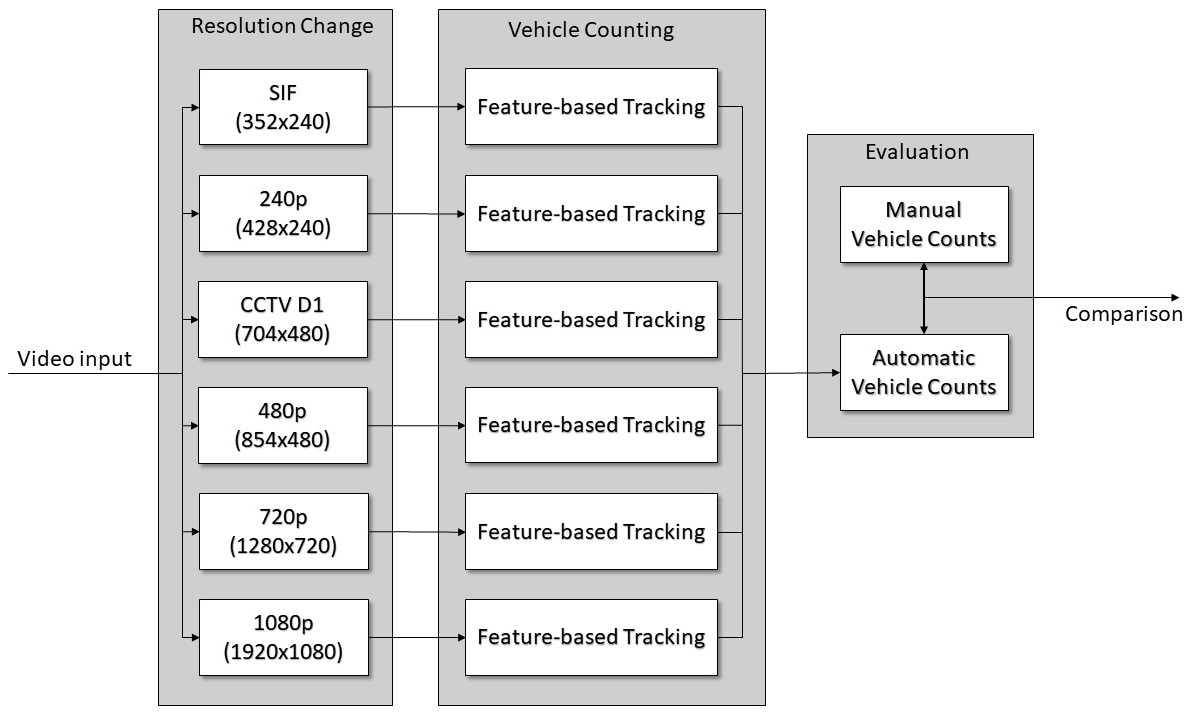
\includegraphics[width=0.75\textwidth]{Figuras/fig1.jpg}
	\caption{Flowchart of the proposed method.}
	\label{fig:fig1}
\end{figure}

For a better understanding of the traking algorithm used to create the automatic count of vehicles, a flowchart of the method proposed by \citet{marcomini2018} can be seen in Figure~\ref{fig:fig0}. All videos have their perspective changed, to eliminate the influence of different camera angles. The resulting frame has it's background removed, using an adaptive Gaussian mixture model known as MOG2 \citep{zivkovic2004improved}, and features are detected. All detected features are tracked and grouped in vehicle hypothesis, which is then extracted as data files from the system.

\begin{figure}[h]
	\centering
	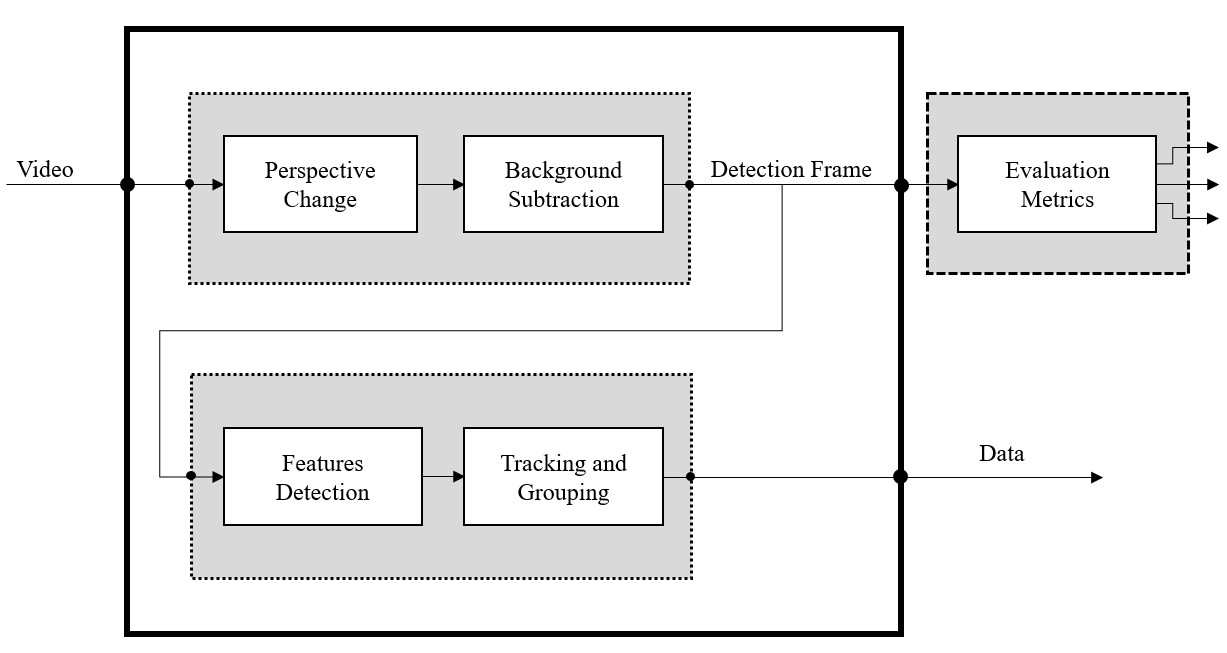
\includegraphics[width=0.75\textwidth]{Figuras/fig0.jpg}
	\caption{Flowchart of the detection algorithm based on \citet{marcomini2018}.}
	\label{fig:fig0}
\end{figure}

All functions on the used algorithm are implemented in Python 2.7, using the OpenCV 2.4 library \citep{OpenCV2019}.

\section{DATA}
In total, we analyzed 32 videos for each resolution presented in Figure 1, totaling 394 minutes of footage recorded on the same day. The cameras were placed on top of a footbridge, over an avenue, with no intervention on the local traffic and centered on the line dividing lanes. All original videos have a resolution of 1920x1080 pixels, recorded at 30 frames per second (FPS).

Half the videos (16) were recorded with the camera pointing to the same direction of the traffic flow. That way, vehicles appear on the bottom of the frame and vanish on the top. The other 16 videos were recorded against traffic flow, at the top of the same footbridge, at the same time. Vehicles enter the frame on the top and leave on the bottom. Examples of angle and direction of the videos can be seen in Figure~\ref{fig:fig2}.

\begin{figure*}[!htbp]
	\begin{minipage}[t]{0.5\textwidth}		
		\centering
		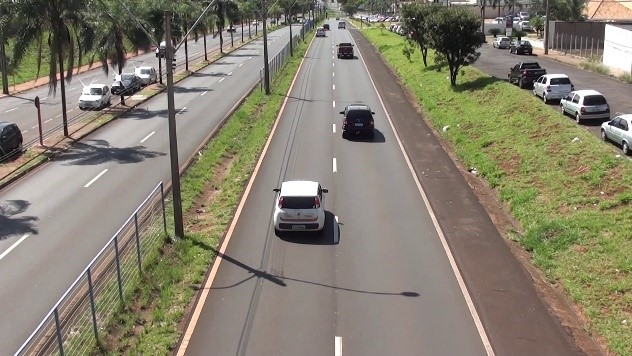
\includegraphics[width=0.985\textwidth]{Figuras/fig2a.jpg}
		\label{fig:sub:subfigure2a}
		\vspace{0.025\textwidth}
	\end{minipage}
	\hspace{\fill}
	\begin{minipage}[t]{0.5\textwidth}
		\centering
		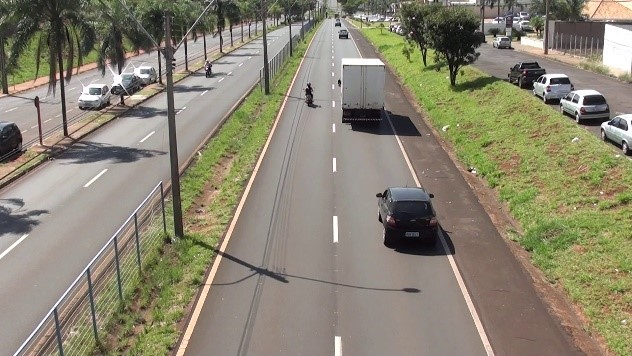
\includegraphics[width=0.985\textwidth]{Figuras/fig2b.jpg}
		\label{fig:sub:subfigure2b}
		\vspace{0.025\textwidth}
	\end{minipage}
	\begin{minipage}[t]{0.5\textwidth}
		\centering
		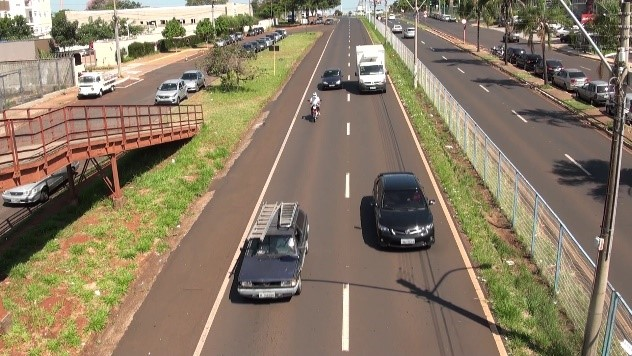
\includegraphics[width=0.985\textwidth]{Figuras/fig3c.jpg}
		\label{fig:sub:subfigure3c}
	\end{minipage}
	\hspace{\fill}
	\begin{minipage}[t]{0.5\textwidth}
		\centering
		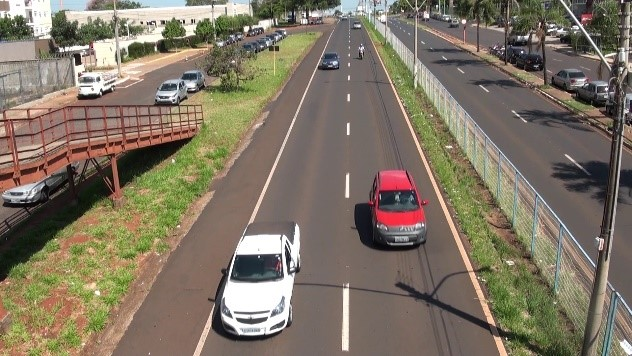
\includegraphics[width=0.985\textwidth]{Figuras/fig3d.jpg}
		\label{fig:sub:subfigure3d}
	\end{minipage}
	\caption{Videos recorded both in the same direction and against the traffic flow.}
	\label{fig:fig2}
\end{figure*}

It was important to keep conditions constant through all recorded videos, so we would be able to isolate the possible effects only of the resolution changes.

\section{RESOLUTION CHANGE}
Given that the original videos were recorded at 1920x1080 pixels, it was necessary to create other instances of the same files, but with different resolutions. For that purpose, we implemented a method in Python using the functions available in the OpenCV library. More specifically, we used the function cv2.resize(), which takes as parameters the frame to be converted and the new desired size, with the option to choose from a range of interpolations. The default conversion algorithm uses a geometric transformation based on bilinear interpolation \citet{OpenCV2016}. On this conversion, the intensity of the pixel to be scaled up or down, pixel (x,y) on Figure~\ref{fig:fig4}, is determined based on four diagonal closest neighbors on a 2 by 2 window, pixels (x1,y1), (x2,y2), (x3,y3), (x4,y4) \citep{Cambridge2019}.

\begin{figure}[h]
	\centering
	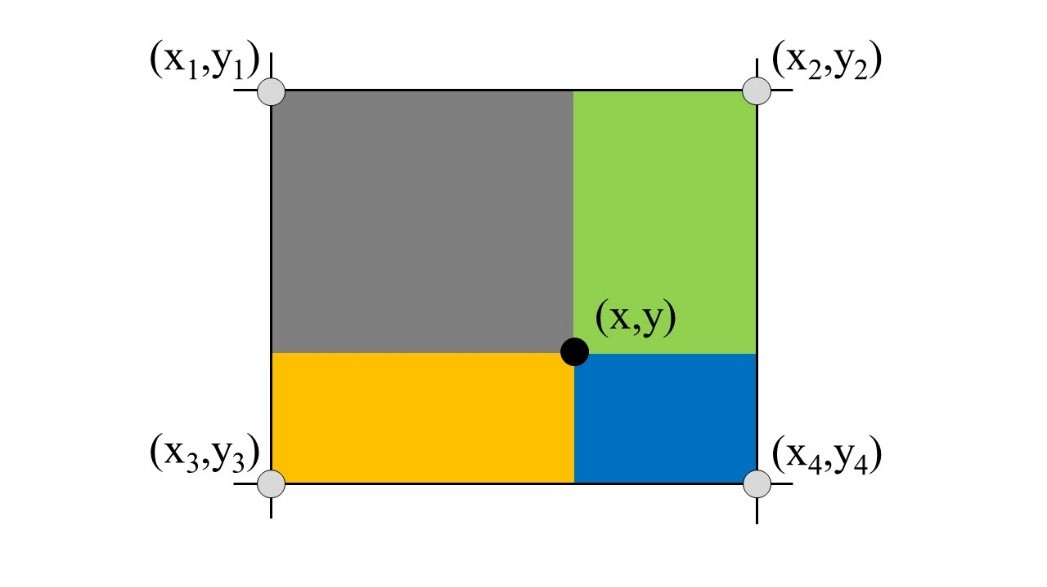
\includegraphics[width=0.6\textwidth]{Figuras/fig4.jpg}
	\caption{Undetermined intensity pixel (x,y) and closest neighbors.}
	\label{fig:fig4}
\end{figure}

The hypothesis of this paper is to analyze the effects on vehicle detection when the resolution changes. Therefore, it's important to isolate the changes from other common variables on traffic images, such as lighting and vehicle sizes. By using the same videos, but converted to several different resolutions, we aim to reduce the effects of grouping errors that different vehicles sizes have on feature-based tracking algorithms. Since the only variable that changes between the videos is the resolution, the difference in vehicle counting can be associated with the resolution change.

\section{VEHICLE COUNTING}
In order to compare the performance of several different resolutions, we manually counted vehicles in all 32 videos and registered the number of vehicles at every minute mark. An example of the procedure can be seen in Table~\ref{tab:tab1}.

\begin{table}[h]
	\centering
	\caption{Manual vehicle counts grouped by minute.}
	\begin{tabular}{r|rS|rS|rS} 
		\hline
		\multicolumn{1}{l}{} & \multicolumn{2}{c}{Video 1} & \multicolumn{2}{c}{Video 2} & \multicolumn{2}{c}{Video 3}  \\ 
		\hline
		Time (min)&Frame no. &{Vehicles}                   &Frame no. &{Vehicles}      &Frame no. &{Vehicles}\\ 
		\hline
		1		  &1793   &11                  &1800   &13                   &1774   &16                    \\
		2		  &3630   &12                  &3640   &14                   &3602   &11                    \\
		3		  &5395   &2                   &5494   &11                   &5406   &17                    \\
		4		  &7313   &13                  &7296   &13                   &7247   &12                    \\
		5		  &8979   &11                  &9127   &13                   &9065   &12                    \\
		6		  &10837  &11                  &10843  &12                   &10792  &15                    \\
		7		  &12607  &11                  &12664  &12                   &12573  &10                    \\
		8		  &14401  &10                  &14410  &15                   &14528  & 18                   \\
		9		  &16205  &4                   &16158  &13                   &16400  &16                    \\
		10		  &17986  &11                  &18013  &17                   &18036  &15                    \\
		11		  &19878  &13                  &19802  &19                   &19788  &9                    \\
		12		  &21581  &10                  &21596  &12                   &21580  &11                    \\
		13		  &23788  &19                  &23653  &10                   &24193  &9                    \\ 
		\hline
		\multicolumn{1}{l}{} &  &138                   &  &174                   &  &171                   
	\end{tabular}
    \label{tab:tab1}
\end{table}

By using the values for each minute on our manual count to compare with the automatic count for each resolution, we were able to extract an absolute average detection error (using Equation 1) for each video. This absolute average detection error is calculated based only on positive numbers, so if the error observed on a specific minute is negative (automatic count smaller then manual count), the absolute value will be used. For example, in Table~\ref{tab:tab2}, it is possible to notice that all detection errors are positive numbers. Thus, by calculating the average of all values, the total detection error on that video will be 6.5\%. By using this method instead of counting the total number of vehicles on the entire video and comparing the total values, we aim to diminish the effect of accumulated errors. For instance, if the algorithm counts one less vehicle at a minute and then counts one extra vehicle later, the total detection error would be 0\%. By separating each minute, we compute this localized error in the total.

\begin{equation}
AbsError = \frac{\sum_{1}^{m}\frac{n_{man}}{n_{aut}}}{m}
\end{equation}
\begin{variaveis}
	m &	Video duration, in minutes; \\
	n_{man} & Manual vehicle count; \\
	n_{aut} & Automatic vehicle count.
\end{variaveis}

\begin{table}[h]
	\centering
	\caption{Detection errors on one 352~x~240 resolution video.}
	\begin{tabular}{rrSSS[table-format=2.1]} 
		\hline
		Time (min)&Frame no.  &{Manual Count}  &{Automatic 352x240}  &{Detection Error}   \\ 
		\hline
		1&1793    &11  &11  &0.0\%   \\
		2&3630    &12  &12  &0.0\%   \\
		3&5395    &2   &2   &0.0\%   \\
		4&7313    &13  &14  &7.7\%   \\
		5&8979    &11  &12  &9.1\%   \\
		6&10837   &11  &10  &9.1\%   \\
		7&12607   &11  &12  &9.1\%   \\
		8&14401   &10  &9   &10.0\%   \\
		9&16205   &4   &4   &0.0\%   \\
		10&17986  &11  &10  &9.1\%   \\
		11&19878  &13  &13  &0.0\%   \\
		12&21581  &10  &12  &20.0\%   \\
		13&23788  &19  &17  &10.5\%   \\ 
		\hline
		&  &  &  &6.5\%  
	\end{tabular}
    \label{tab:tab2}
\end{table}

\section{RESULTS}
In order to easily observe the distribution of detection error of all 32 videos, grouped by resolution, histogram plots can be seen in Figure~\ref{fig:fig5a}.

\begin{figure*}[!htbp]
	\begin{minipage}[t]{0.5\textwidth}		
		\centering
		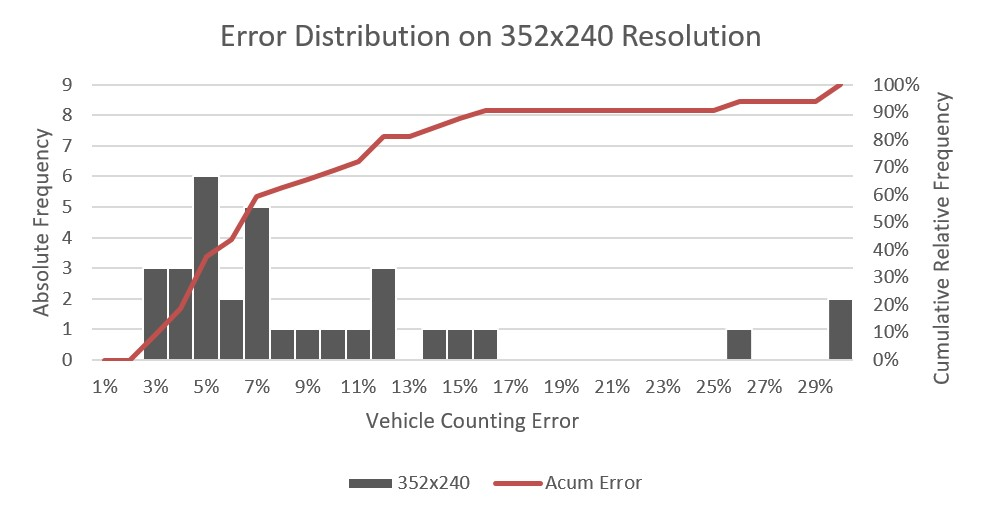
\includegraphics[width=0.985\textwidth]{Figuras/graf1.jpg}
		\label{fig:sub:subfigure5aa}
		\vspace{0.025\textwidth}
	\end{minipage}
	\hspace{\fill}
	\begin{minipage}[t]{0.5\textwidth}
		\centering
		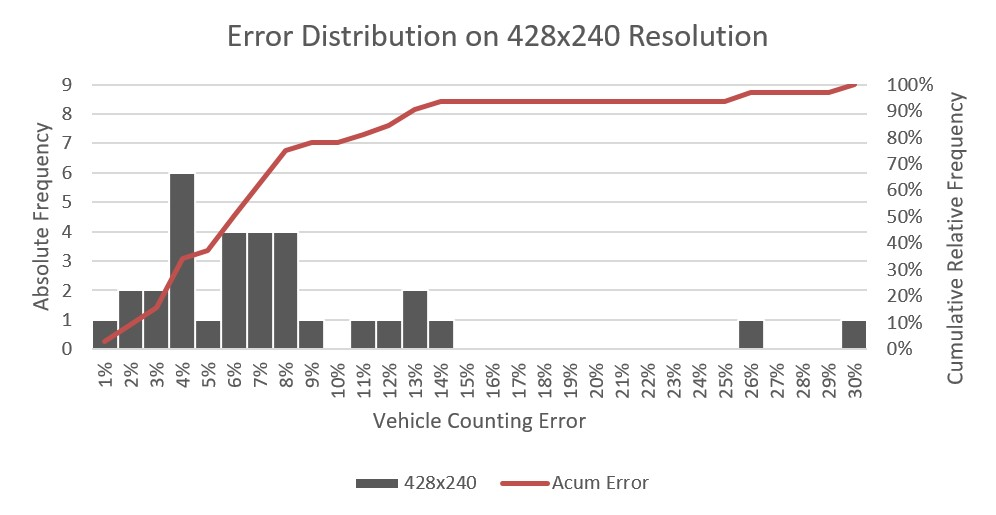
\includegraphics[width=0.985\textwidth]{Figuras/graf2.jpg}
		\label{fig:sub:subfigure5ab}
		\vspace{0.025\textwidth}
	\end{minipage}
	\begin{minipage}[t]{0.5\textwidth}
		\centering
		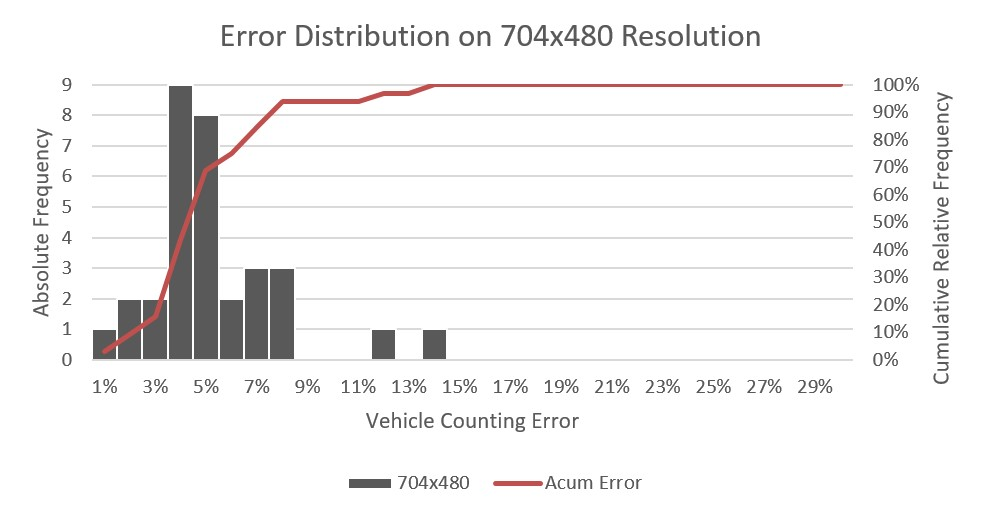
\includegraphics[width=0.985\textwidth]{Figuras/graf3.jpg}
		\label{fig:sub:subfigure5ac}
	\end{minipage}
	\hspace{\fill}
	\begin{minipage}[t]{0.5\textwidth}
		\centering
		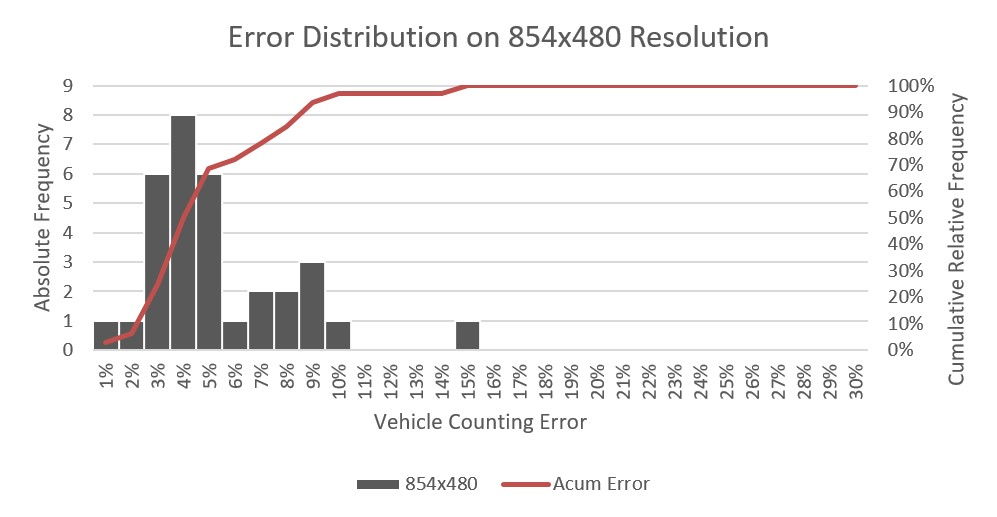
\includegraphics[width=0.985\textwidth]{Figuras/graf4.jpg}
		\label{fig:sub:subfigure5ad}
	\end{minipage}
	\begin{minipage}[t]{0.5\textwidth}		
		\centering
		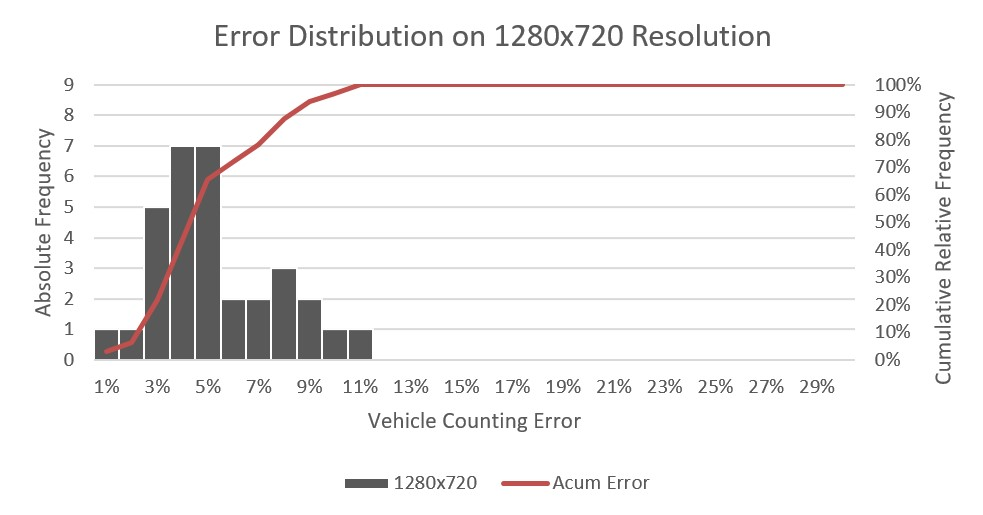
\includegraphics[width=0.985\textwidth]{Figuras/graf5.jpg}
		\label{fig:sub:subfigure5ae}
		\vspace{0.025\textwidth}
	\end{minipage}
	\hspace{\fill}
	\begin{minipage}[t]{0.5\textwidth}
		\centering
		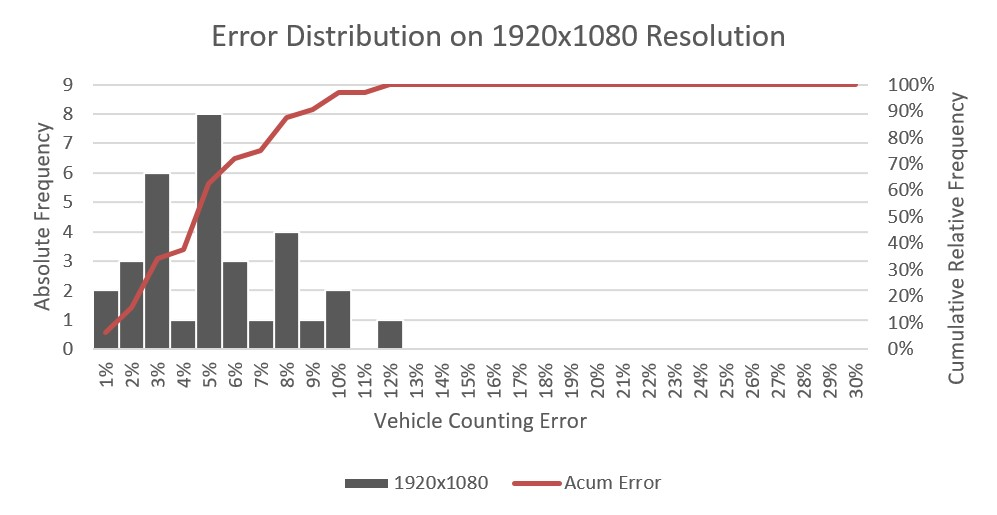
\includegraphics[width=0.985\textwidth]{Figuras/graf6.jpg}
		\label{fig:sub:subfigure5af}
		\vspace{0.025\textwidth}
	\end{minipage}
	\caption{Histogram plots of vehicle counting errors for each resolution.}
	\label{fig:fig5a}
\end{figure*}

Based only on the histograms, it's possible to notice that detection errors tend to concentrate more on smaller values on intermediate and high resolutions, from 704~x~480 to 1920~x~1080, resulting in less detection errors overall.

The descriptive statistics of all detection errors can be seen on the boxplot graphic in Figure~\ref{fig:fig5}. Each boxplot represents data from all videos of one resolution. To calculate the values, such as first quartile, average resolution error, and third quartile, data from all 32 videos of each resolution was used, i.e., to extract the average resolution error value for the resolution 352~x~240, we summed all detection errors of all videos on that resolution and divided the value by the number of videos. The equation used can be seen in Equation~2. All different vehicles categories - motorcycles, cars, trucks, busses - are grouped together on the counts, since the objective of this paper is to analyze the effect of resolution changes on the overall detection rate, although the variation on vehicle's sizes present a challenge for grouping features, as demonstrated by \citet{marcomini2018} and others.

\begin{minipage}[t]{1\textwidth}
	\begin{equation}
	AvgResErr= \frac{\sum_{1}^{n_{vid}}{AbsError}}{n_{vid}}
	\end{equation}
	\begin{variaveis}
		AvgResErr & Average detection error of a specific resolution;\\
		n_{vid}   & number of videos (32); \\
		AbsError  & Absolute average error, from Equation~1.
	\end{variaveis}
\end{minipage}

\begin{figure}[h]
	\centering
	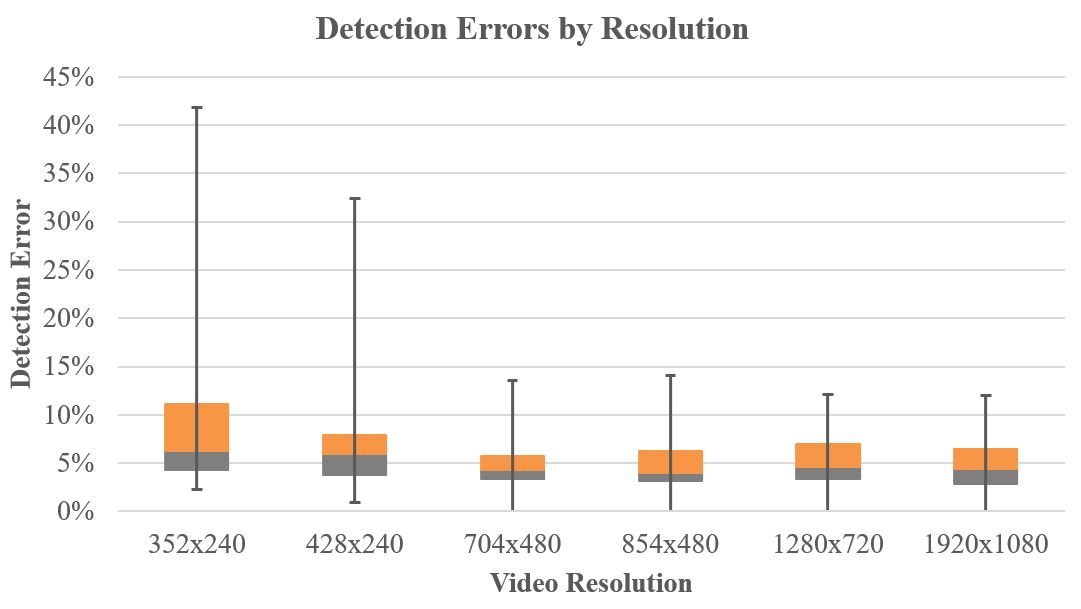
\includegraphics[width=0.6\textwidth]{Figuras/fig5.jpg}
	\caption{Boxplot of the detection errors grouped by resolution.}
	\label{fig:fig5}
\end{figure} 

It is possible to notice that at the lowest evaluated resolution, 352~x~240, 75\% (3º quartile) of the encountered detection errors happened below the 11\% margin. In other words, in 75\% of all evaluated videos, the feature-based tracking algorithm incurred errors that were lower or equal to 11\% in the counting process. Although that is not a bad tracking and counting performance, this result is still the worst observed in all evaluated resolutions.

The best result can be seen on the 704~x~480 resolution, where 75\% of all detection errors were below 6\%. Two other resolutions also presented a satisfying performance. At 854~x~480 and 1920~x~1080, detection errors were equivalent between each other.

The results indicate that low resolutions may incur in greater detection errors. Since vehicles are represented by a small number of pixels, the feature-based tracking algorithm suffers to encounter relevant points to track. However, the opposite is not true. High resolutions, in our tests, did not outperform other lower resolutions. 

In order to validate the null hypothesis that resolutions do not present a difference between each other, a Kolmogorov-Smirnov test was applied in the sample. Since 32 videos have been tested, our sample size is 32. For that sample size, the critical value to $\alpha = 5\%$ is $D_{critical} = 0.24$. If the critical value is lower than 0.24, it's not possible to reject the null hypothesis that the error distribution between the two videos are different. The results of the tests can be seen in Table~\ref{tab:tab3}  

\begin{table}[h]
	\centering
	\caption{Comparison for Kolmogorov-Smirnov results. A green check denotes equal distributions while a red check denotes different distributions.}
	\begin{tabular}{rcccccc} 
		\hline
		\multicolumn{7}{c}{\textbf{Kolmogorov-Smirnov Test ($D_{critical}=0.24$)}} \\ 
		\hline
		         &352x240 &428x240    			  &704x480 					&854x480   				  &1280x720 				& 1920x1080   			  \\
		352x240  &-		  &\textcolor{ao}{\cmark} &\textcolor{bred}{\xmark} &\textcolor{bred}{\xmark} &\textcolor{bred}{\xmark} &\textcolor{bred}{\xmark} \\
		428x240  &-       &-  		  			  &\textcolor{bred}{\xmark} &\textcolor{bred}{\xmark} &\textcolor{bred}{\xmark} &\textcolor{bred}{\xmark} \\
		704x480  &-		  &-          			  &-  		 			    &\textcolor{ao}{\cmark}   &\textcolor{ao}{\cmark}   &\textcolor{ao}{\cmark}   \\
		854x480  &-		  &-         			  &- 		 				&-  		 			  &\textcolor{ao}{\cmark}   &\textcolor{ao}{\cmark}   \\
		1280x720 &-	      &-         			  &- 		 				&-  		 			  &- 		 			    &\textcolor{ao}{\cmark}   \\
		\hline
	\end{tabular}
	\label{tab:tab3}
\end{table}

For lower resolutions (352~x~240 and 428~x~240), the Kolmogorov-Smirnov test passed, so it’s not possible to reject the hypothesis that the error distributions are different. But, when compared to higher resolutions, the test failed, indicating that there is a difference between higher resolutions and lower ones.

When comparing the average processing times for each resolution, the two higher resolutions tested, 1280~x~720 and 1920~x~1080, took more time to process all video files but did not had a proportional gain in vehicle detection. At our highest resolution, 1920~x~1080, the algorithm took, on average, 422 minutes to process 394 minutes of footage, exceeding the recording time in 7\%, as can be seen in Figure~\ref{fig:fig6}.  

\begin{figure}[h]
	\centering
	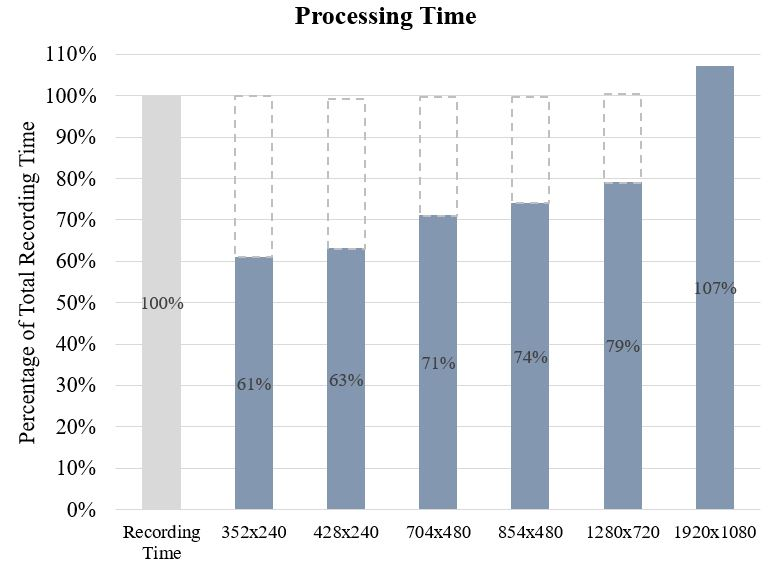
\includegraphics[width=0.6\textwidth]{Figuras/fig6.jpg}
	\caption{Total average processing time of different resolutions compared to the total time of evaluated footage.}
	\label{fig:fig6}
\end{figure}

In conclusion, our tests suggest that low resolutions, such as 352~x~240 or 428~x~240, are not recommended for a feature-based tracking algorithm, although its processing time is significantly lower than other resolutions. Not enough pixels are used to represent vehicles and, therefore, feature detection and tracking are impaired. High-definition resolutions do not suffer from this issue. However, greater amount of pixels do not represent a significant detection gain over intermediate resolutions, such as 704~x~480 or 854~x~480. Furthermore, HD resolutions incur in greater processing times. Intermediate resolutions, on the other hand, showed an equivalent detection rate to high resolutions, with a smaller processing time. Based on these results, it is recommended to use intermediate resolutions, such as 704~x~480 or equivalent in other aspect ratios, to decrease processing times while keeping the detection error rate at similar levels with higher resolutions.  

\section{CONCLUSION}
The hypothesis proposed in this paper was that there is no impact on vehicle detection of a feature-based tracking algorithm using different video resolutions. This hypothesis was rejected for videos with smaller resolutions, but accepted for higher resolutions. We analyzed 32 videos, comprising of 394 minutes of footage, comparing the results of automatic vehicle counts to manual vehicle counts. As a result, our tests suggest that the use of low resolutions have a bad impact on feature-based tracking algorithms, incurring in greater detection errors. Since less pixels are used to draw vehicles, farther vehicles are grouped together in one single object. We also concluded that high resolutions, such as HD or full HD, do not represent a gain in vehicle detection and have a negative impact on processing times. Consequently, intermediate resolutions, such as 480p (704~x~480 or 854~x~480), are recommended for feature-based tracking algorithms and present the best results in our tests, both on detection rate and processing time.

\begin{footnotesize}
	\footnotesize{\textbf{Acknowledgements}}
	\setlength{\parskip}{0pt} \par
	\footnotesize
	\begin{SingleSpace}
		%TEXTO DO AGRADECIMENTO	
		The authors would like to thank São Carlos School of Engineering, for all the support. This study was financed in part by the Coordenação de Aperfeiçoamento de Pessoal de Nível Superior - Brasil (CAPES) - Finance Code 001.		
		%FIM DO TEXTO DO AGRADECIMENTO
		\setlength{\parskip}{12pt}
	\end{SingleSpace}
\end{footnotesize}


%Fim do texto.

%%%%NOTA: As citações da abnt, logo abaixo, não estão funcionando.
%\nocite{abnt2002a}
%\nocite{abnt2002b}
%\nocite{abnt2003a}
%\nocite{abnt2003b}

\renewcommand{\bibsection}{
	\setsecheadstyle{\bfseries \footnotesize \uppercase}
	{\section*{References}}}
\renewcommand{\bibfont}{\footnotesize}
%\bibliographystyle{apacite}
\bibliographystyle{bib/chicago-br.bst}
\setlength{\bibsep}{0pt}        % elimina espaços entre referências

\bibliography{bib/Referencias.bib}

\begin{minipage}[]{\linewidth}
	\footnotesize
	\setlength{\parskip}{0pt}
	\noindent\rule[1pt]{\linewidth}{1pt}
	Leandro Arab Marcomini (leandro.marcomini@usp.br) \\
	André Luiz Cunha (alcunha@usp.br) \\
	Department of Transport Engineering, São Carlos School of Engineering, University of São Paulo\\
	1465 Dr. Carlos Botelho Avenue – São Carlos, SP, Brasil \\
\end{minipage}

\end{document}